\section{Modelos de Mistura Gaussiana}
\label{sec:gmm}

\contentscurrent

\begin{frame}
\frametitle{Definição}
\begin{description}\itemsep6pt
    \item[GMM] $\postpdf{\dvec{x}}{\lambda} = \sum_{i=1}^M w_i\pdfi{\dvec{x}}$
    \item[Gaussiana] $\pdf{\dvec{x}} = \dgaussian{x}{\mu}{\Sigma}$
    \item $\lambda = \{(w_i, \dvec{\mu}_i, \dvec{\Sigma}_i)\}, i = 1, ..., M$
    \item $\dvec{\Sigma}$ diagonal $\implies \dvec{\sigma}^2$
    \item Dada uma sequência $\boldsymbol{X}$
    \begin{itemize}\itemsep4pt
        \item $\postpdf{\boldsymbol{X}}{\lambda} = \prod_{t=1}^T \postpdf{\dvec{x}_t}{\lambda}.$
        \item Função não linear de $\lambda$
        \item Estimar com o Expectation-Maximization (EM)
    \end{itemize}
\end{description}
\end{frame}

\subsection{EM}

\begin{frame}
\frametitle{Expectation-Maximization}
\begin{description}\itemsep6pt
    \item Estimar $\lambda^{(k+1)}$ a partir de $\lambda^{k}$
    \item Obedecer $\postpdf{\boldsymbol{X}}{\lambda^{(k+1)}} \geq \postpdf{\boldsymbol{X}}{\lambda^{(k)}}$
    \item Calcular \emph{E-Step} e \emph{M-Step} para cada $k$ até convergir
    \item[E-Step] $\postprob{i}{\dvec{x}_t} = \frac{w_i p_i(\dvec{x}_t)}{\sum_{k=1}^M w_k p_k(\dvec{x}_t)}$
    \item[M-Step] Adaptar os parâmetros
    \begin{description}\itemsep6pt
        \item[Pesos] $\overline{w}_i = \frac{1}{T} \sum_{t=1}^T \postprob{i}{\dvec{x}_t, \lambda}$
        \item[Médias] $\overline{\dvec{\mu}}_i = \frac{\sum_{t=1}^T \postprob{i}{\dvec{x}_t, \lambda} \dvec{x}_t}{\sum_{t=1}^T \postprob{i}{\dvec{x}_t, \lambda}}$
        \item[Variâncias] $\overline{\dvec{\sigma}}_i^2 = \frac{\sum_{t=1}^T \postprob{i}{\dvec{x}_t, \lambda} \dvec{x}_t^2}{\sum_{t=1}^T \postprob{i}{\dvec{x}_t, \lambda}} - \overline{\dvec{\mu}}_i^2$
    \end{description}
\end{description}
\end{frame}

\begin{frame}
\frametitle{Expectation-Maximization}
\begin{figure}[ht]
    \centering
    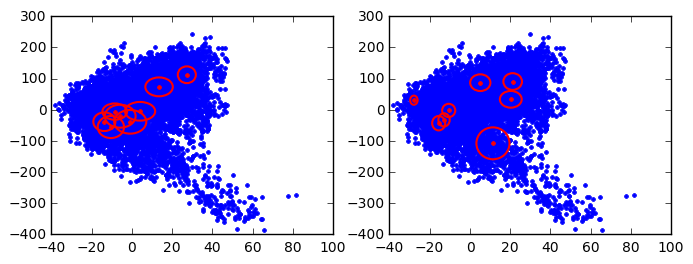
\includegraphics[width=0.75\textwidth]{em_algorithm}
\end{figure}

\begin{description}
    \item $M = 8$ e $\Delta = 0$
    \item[Inicialização] \emph{k-means} com 1 iteração
    \item[Limiar] $10^{-3}$
\end{description}
\end{frame}

\subsection{UBM}

\begin{frame}
\frametitle{Universal Background Model}
\begin{description}
    \item Utiliza locuções de todos os locutores registrados
    \item Realça características comuns
    \item $\boldsymbol{X}$ específico a $\mathcal{S} \implies \uparrow \Lambda(\boldsymbol{X})$
    \item Escolhido o tipo $(b)$
\end{description}

\begin{figure}[ht]
    \centering
    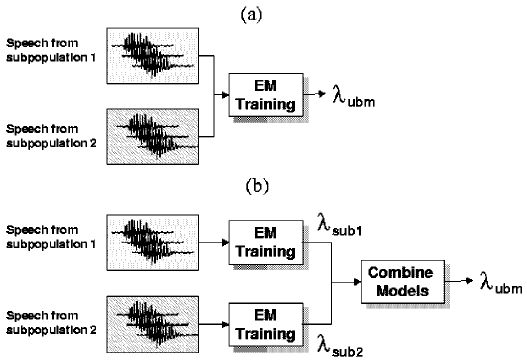
\includegraphics[width=0.5\textwidth]{ubm-diagram}
\end{figure}
\end{frame}

\subsection{AGMM}

\begin{frame}
\frametitle{Adapted Gaussian Mixture Model}
\begin{description}
    \item[Adaptação] $\lambda_{bkg}$ treinado $\implies \lambda_j$ para cada $\mathcal{S}_j$
    \item Modelagem mais rápida que EM
    \item Composto de \emph{E-Step} e \emph{MAP-Step}
    \item[E-Step] Semelhante ao \emph{E-Step} do EM
    \begin{itemize}\itemsep4pt
        \item $n_i = \sum_{t=1}^{T} \postprob{i}{\dvec{x}_t}
    \label{eq:n_i}$
        \item $E_i(\dvec{x}) = \frac{1}{n_i} \sum_{t=1}^{T} \postprob{i}{\dvec{x}_t} \dvec{x}_t$
        \item $E_i(\dvec{x}^2) = \frac{1}{n_i} \sum_{t=1}^{T} \postprob{i}{\dvec{x}_t} \dvec{x}_t^2$
    \end{itemize}
    \item[MAP-Step] Adapta os parâmetros
    \begin{description}\itemsep4pt
        \item[Pesos] $\hat{w_i} = [\alpha_i n_i / T + (1 - \alpha_i)w_i]\gamma$
        \item[Médias] $\hat{\dvec{\mu}_i} = \alpha_i E_i(\dvec{x}) + (1 - \alpha_i)\dvec{\mu}_i$
        \item[Variâncias] $\hat{\dvec{\sigma}_i}^2 = \alpha_i E_i(\dvec{x}^2) + (1 - \alpha_i)(\dvec{\sigma}_i^2 + \dvec{\mu}_i^2) - \hat{\dvec{\mu}_i}^2$
    \end{description}
\end{description}
\end{frame}

\begin{frame}
\frametitle{Adapted Gaussian Mixture Model}
\begin{description}
    \item $\gamma$ normaliza os pesos
    \item[Coeficiente] $\alpha_i = \frac{n_i}{n_i + r}$
    \begin{itemize}
        \item $\alpha_i \to 0 \implies$ manter os antigos parâmetros
        \item $\alpha_i \to 1 \implies$ adaptar para os novos parâmetros
    \end{itemize}
\end{description}

\begin{figure}[ht]
    \centering
    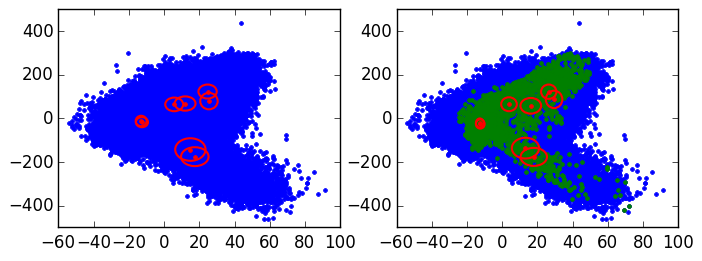
\includegraphics[width=0.75\textwidth]{adapted_wmv}
\end{figure}

\begin{description}
    \item Pesos, médias e variâncias adaptados
\end{description}
\end{frame}

\subsection{FGMM}

\begin{frame}
\frametitle{Fractional Gaussian Mixture Model}
\begin{description}
    \item GMM com $\dvec{\Sigma}$ fracionário
    \pause
    \begin{itemize}\itemsep4pt
        \item $\sigma^2 = E[(X^r - \mu^r)^2]$
        \item $\overline{\dvec{\sigma}}_i^2 = \frac{\sum_{t=1}^T \postprob{i}{\dvec{x}_t, \lambda} (\dvec{x}_t^r - \overline{\dvec{\mu}}_i^r)^2}{\sum_{t=1}^T \postprob{i}{\dvec{x}_t, \lambda}}$
        \pause
    \end{itemize}
    \item[Problema] $\mathbb{C}$
    \pause
    \begin{description}\itemsep4pt
        \item[Antes] $c_n = c_n + (1 - \min_t c_{n,t})$
        \item[Depois] $\mu_n = \mu_n - (1 - \min_t c_{n,t})$
        \pause
    \end{description}
\end{description}

\begin{figure}[ht]
    \centering
    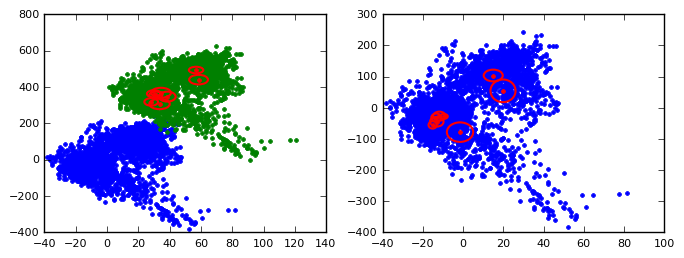
\includegraphics[width=0.75\textwidth]{em_algorithm_r095}
\end{figure}
\end{frame}

\begin{frame}
\frametitle{Fractional Gaussian Mixture Model}
\begin{description}
    \item Piora quando $r \downarrow$
\end{description}

\begin{figure}[ht]
    \centering
    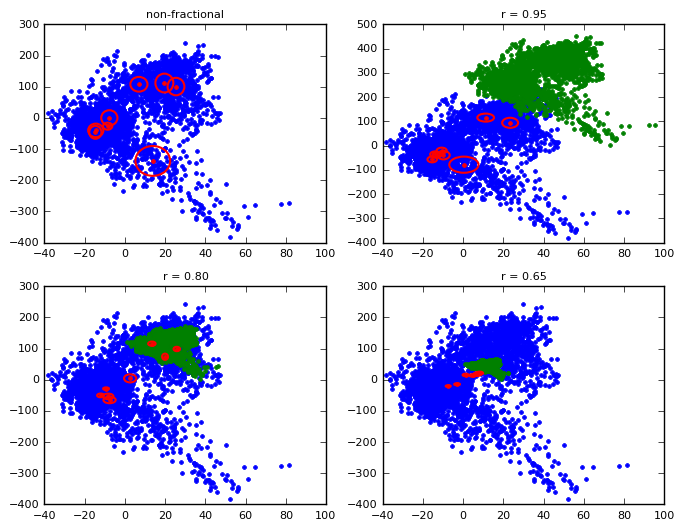
\includegraphics[width=0.65\textwidth]{frac-em-r-down}
\end{figure}
\end{frame}

\begin{frame}
\frametitle{Fractional Gaussian Mixture Model}
\begin{description}
    \item E quando $r \uparrow$
\end{description}

\begin{figure}[ht]
    \centering
    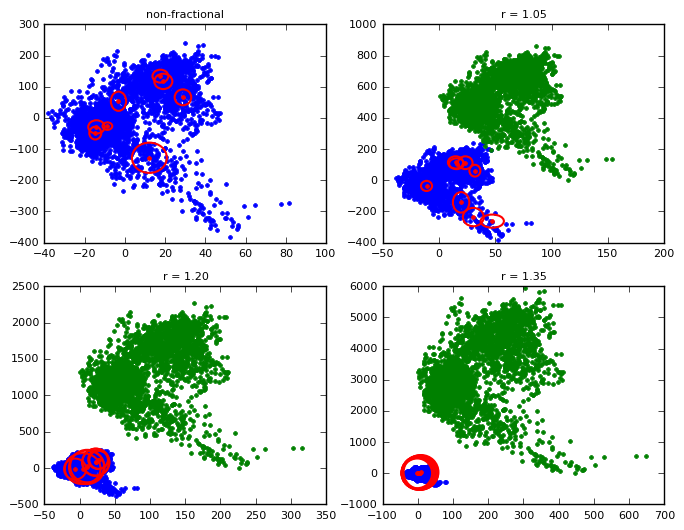
\includegraphics[width=0.65\textwidth]{frac-em-r-up}
\end{figure}
\end{frame}